\section{Conclusion}

\begin{frame}{Open access and education}
    \vspace{-4em}
    \begin{itemize}
        \item Open access: a dedicated portal planned
        \item Education: \textcolor{blue}{\texttt{astroparticle.online}}
    \end{itemize}
    \centering
    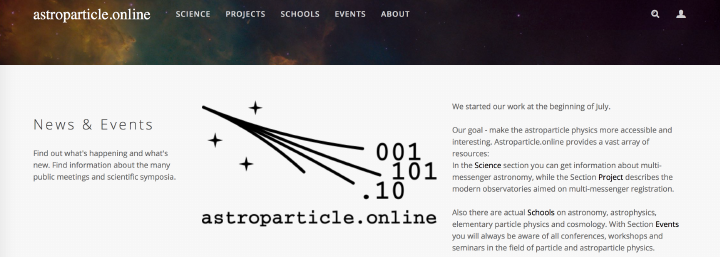
\includegraphics[width=0.85\textwidth]{pics/astro_onl.png}
\end{frame}

\begin{frame}{Outlook}
\textcolor{red}{Improve the translation quality!!!}
    \begin{itemize}
%     \item mdl
%     \item kcdc
%     \item Нужны инструменты совместного доступа к данным различных экспериментов и эффективный бережный менеджмент этих больших объемов данных
%     \item Консоциум gradlc предлагает концепцию дата инжиниринга в области астропартикл физикс, основанный на уже kcdc. 
%     \item В данный момент производятся работы по созданию aggregation data server'a и совместному анализу данных из экспериментов kascade и taiga;
% \item Доступ к ресурса проекта на данный момент частично предоставлен через портал astroparticle.online.

        \item Need for tools to share data from various experiments and to manage these large volumes of data with care
        \item The gradlc consortium offers the concept of date engineering in the field of astroparticle physics, based on kcdc already. 
        \item The aggregation data server and the joint analysis of data from kascade and taiga experiments are currently being developed;
        \item Access to the project resource is now partially provided through the astroparticle.online portal.

    \end{itemize}
\end{frame}

% \subsection{The end}
% \begin{frame}{}
%     \begin{center}
%         \textcolor{kit-green100}{\Huge Thank you\\for your attention!\vspace{1em}}  
%         \Large Any questions?
%     \end{center}
% \end{frame}
